\chapter{Derived Morita Theory for Noncommutative Projective Schemes} \label{section: morita for NCP}

Let \(A\) and \(B\) be as in Chapter~\ref{chapter: background on NCP}. We want to extend the ideas from Chapter~\ref{chapter: graded Morita} to cover dg-enhancements of \(\mathrm{D}(\QGr{A})\). 

\section{Vanishing of a tensor product} \label{subsection: vanishing of tensor}

We recall a particularly nice type of property of objects in the setting of compactly generated triangulated categories.
In the sequel, many of our properties will be of this type, so we give this little gem a name.

\begin{definition} \label{definition: run the jewels}
  Let \(\D\) be a compactly generated triangulated category.
  Let \(\mathtt{P}\) be a property of objects of \(\D\). 
  We say that \(\mathtt{P}\) is \textbf{RTJ} if it satisifies the following three conditions.
  \begin{itemize}
  \item Whenever \(A \to B \to C\) is a triangle in \(\D\) and \(\mathtt{P}\) holds for \(A\) and \(B\), then \(\mathtt{P}\) holds for \(C\). 
  \item If \(\mathtt{P}\) holds for \(A\), then \(\mathtt{P}\) holds for the translate \(A[1]\).
  \item Let \(I\) be a set and \(A_i\) be objects of \(\D\) for each \(i \in I\). If \(\mathtt{P}\) holds for each \(A_i\), then \(\mathtt{P}\) holds for \(\bigoplus_{i \in I} A_i\). 
  \end{itemize}
\end{definition}

\begin{proposition} \label{proposition: RTJ properties}
  Let \(\mathtt{P}\) be an RTJ property that holds for a set of compact generators of \(\D\). Then \(\mathtt{P}\) holds for all objects of \(\D\).
\end{proposition}

\begin{proof}
  Let \(P\) be the full triangulated subcategory of objects for which \(\mathtt{P}\) holds. Then \(P\)
  \begin{itemize}
  \item contains a set of compact generators,
  \item is triangulated, and
  \item is closed under formation of coproducts. 
  \end{itemize}
  Thus, \(P\) is all of \(\D\). 
\end{proof}


\begin{definition} \label{definition: tensor vanishing}
  Let \(M\) be a complex of left graded \(A\)-modules and let \(N\) be a complex of right graded \(A\)-modules. We say that the pair satisfies \(\bigstar(M,N)\) if we have vanishing of the tensor product
  \begin{displaymath}
    \mathbf{R} \tau_{A^\opp} N {\otimes}^{\mathbf{L}}_{\mathcal A} \mathbf{R} Q_A M = 0.
  \end{displaymath}
  If \(\bigstar(M,N)\) holds for all \(M\) and \(N\), then we say that \(A\) satisfies \(\bigstar\). 
\end{definition}

\begin{proposition} \label{proposition: big star condition}
  Assume that \(\mathbf{R}\tau_A\) and \(\mathbf{R}\tau_{A^\opp}\) commute with coproducts. Then \(A\) satisfies \(\bigstar\) if and only \(\bigstar( A(u), A(v) )\) holds for each \(u,v \in \Z\).
\end{proposition}

\begin{proof}
  The necessity is clear, so assume that \(\bigstar(A(u), A(v))\) holds for each \(u,v \in \Z\).
  First, we consider the property \(\bigstar(M, A(v))\) of objects, \(M\), of \(\mathrm{D}(\Gr{A})\).
  It's clear that this is an RTJ property that holds, by assumption, for the set of compact generators, \(\{A(u)\}_{u \in \Z}\).
  Hence \(\bigstar(M,A(v))\) holds for all \(M\) by Proposition~\ref{proposition: RTJ properties}.

  Now fix any object \(M\) of \(\mathrm{D}(\Gr{A})\) and consider the property \(\bigstar(M, N)\) of objects, \(N\), of \(\mathrm{D}(\Gr{A^\opp})\).
  This is again an RTJ property for which \(\bigstar(M,A(v))\) holds for all \(v \in \Z\).
  By Proposition~\ref{proposition: RTJ properties}, \(\bigstar(M,N)\) holds for all N .
  Since the choice of \(M\) was arbitrary, it follows that \(\bigstar(M,N)\) holds for all \(M\) and for all \(N\).
  Therefore \(A\) satisfies \(\bigstar\).
%  The necessity is clear, so assume that \(\bigstar( A(u), A(v) )\) holds for each \(u,v \in \Z\). Note that \(\bigstar(M , A(v))\) holds for all \(v\) is an RTJ property of \(M\) that holds for a set of compact generators \(A(u), u \in \Z\). Thus, by Proposition~\ref{proposition: RTJ properties}, \(\bigstar(M , A(v))\) holds for all \(v\) holds for all \(M\) in \(\mathrm{D}(\Gr{A})\). Similarly, we can consider the property of \(N\) in \(\mathrm{D}(\Gr{(A^\opp)})\): \(\bigstar(M , N)\) holds for all objects \(M\) of \(\mathrm{D}(\Gr{A})\). This is also RTJ so \(\bigstar(M,N)\) holds for all \(M\) and \(N\).
\end{proof}

There are various types of projection formulas.
We record here two which will be useful in the sequel.

\begin{proposition} \label{proposition: projection formula}
  Let \(P\) be a complex of bi-bi \(A\)-modules and let \(M\) be a complex of left graded \(A\)-modules. Assume \(\mathbf{R} \tau_A\) commutes with coproducts. There is a natural quasi-isomorphism
  \begin{displaymath}
    ( \mathbf{R} \tau_A P ) \overset{\mathbf{L}}{\otimes}_{\mathcal A} M \to \mathbf{R} \tau_A \left( P \overset{\mathbf{L}}{\otimes}_{\mathcal A} M \right).
  \end{displaymath}
  Assume \(\mathbf{R} Q_A\) commutes with coproducts. There is a natural quasi-isomorphism
  \begin{displaymath}
    ( \mathbf{R} Q_A P ) \overset{\mathbf{L}}{\otimes}_{\mathcal A} M \to \mathbf{R} Q_A \left( P \overset{\mathbf{L}}{\otimes}_{\mathcal A} M \right).
  \end{displaymath}
\end{proposition}

\begin{proof}
  We treat the \(\tau\) projection formula. The \(Q\) projection formula is analogous. By Corollary~\ref{corollary: Q preserves bimodules}, we see that the tensor product is well-defined. It suffices to exhibit a natural transformation for the underived functors applied to modules to generate the desired natural transformation. Given
  \begin{displaymath}
    \psi \otimes_{\mathcal A} m \in \GR{A}(A/A_{\geq m}, P) \otimes_{\mathcal A} M 
  \end{displaymath}
  we naturally get 
  \begin{align*}
    \widetilde{\psi} : A/A_{\geq m} & \to P \otimes_{\mathcal A} M \\
    a & \mapsto \psi(a) \otimes_{\mathcal A} m. 
  \end{align*}
  Taking the colimit gives the natural transformation.
  
  Let us look at the natural transformation in the case that \(P = A(u) \otimes_k A(v)\) and \(M = A(w)\).
  Recall from Remark~\ref{remark: tensor with twist} that
  \[
  \mathbf{R}\tau_A(P) \otimes_\A^\mathbf{L} A(w) \cong \mathbf{R}\tau_A(P) \otimes_\A A(w) \cong \mathbf{R}\tau_A(P)_{\ast,w} 
  := \bigoplus_{x \in \Z} \mathbf{R}\tau_A(P_{\ast,w})_x
  = \mathbf{R}\tau_A(P_{\ast,w})
  \]
  which is compatible with the natural transformation.
  The property that the natural transformation is a quasi-isomorphism is RTJ in each entry.
  Thus, it holds for all \(P\) and \(M\) by Proposition~\ref{proposition: RTJ properties}.
%  Recall that 
%  \begin{gather*}
%    \left( A(u) \otimes_k A(v) \right) \overset{\mathbf{L}}{\otimes}_{\mathcal A} A(w) \cong \left( A(u) \otimes_k A(v) \right) \otimes_{\mathcal A} A(w) \\ \cong \left( A(u) \otimes_k A(v) \right)_{\ast,w} \cong A(u) \otimes_k A_{v+w}. 
%  \end{gather*}
%  So
%  \begin{displaymath}
%    \mathbf{R}\tau_A \left( \left( A(u) \otimes_k A(v) \right) \overset{\mathbf{L}}{\otimes}_{\mathcal A} A(w) \right) \cong \mathbf{R} \tau_A \left( A(u) \otimes_k A_{v+w} \right)
%  \end{displaymath}
%  while 
%  \begin{gather*}
%    \mathbf{R}\tau_A \left( A(u) \otimes_k A(v) \right) \overset{\mathbf{L}}{\otimes}_{\mathcal A} A(w) \cong \mathbf{R}\tau_A \left( A(u) \otimes_k A(v) \right)_w \\ \cong \mathbf{R}\tau_A \left( (A(u) \otimes_k A(v))_{\ast,w} \right) \cong \mathbf{R}\tau_A \left( A(u) \otimes_k A_{v+w} \right)
%  \end{gather*}
  %which are compatible with the natural transformation. The property that the natural transformation is a quasi-isomorphism is RTJ in each entry. Thus, it holds for all \(P\) and \(N\) by Proposition~\ref{proposition: RTJ properties}. 
\end{proof}

For the hypothesis, recall Definition~\ref{definition: tasty pair}. 

\begin{proposition} \label{proposition: vanishing of tensor}
  Assume \(A\) is truly tasty. Then \(\bigstar\) holds for \(A\).
\end{proposition}

\begin{proof}
  By Proposition~\ref{proposition: big star condition}, it suffices to check \(\bigstar(M,A(v))\) for each \(v\). This is equivalent to \(\bigstar(M,\bigoplus_v A(v))\). Equipping the sum with a bi-bi structure as \(\Delta\), we reduce to checking \(\bigstar(M,\Delta)\). Using Proposition~\ref{proposition: when beta is an isomorphism} and Lemma~\ref{lemma: exact triangles} for \(A\) and \(A^\opp\), we have a natural quasi-isomorphism
  \[\mathbf{R}\tau_{A^\opp} \Delta \overset{\mathbf{L}}{\otimes}_{\mathcal A} \mathbf{R}Q_A M \cong \mathbf{R}\tau_{A} \Delta \overset{\mathbf{L}}{\otimes}_{\mathcal A} \mathbf{R}Q_{A} M.\]
  Using Proposition~\ref{proposition: projection formula}, we have a natural quasi-isomorphism
  \[\mathbf{R}\tau_{A} \Delta \overset{\mathbf{L}}{\otimes}_{\mathcal A} \mathbf{R}Q_{A} M \cong \mathbf{R}\tau_{A} \left( \Delta \overset{\mathbf{L}}{\otimes}_{\mathcal A} \mathbf{R}Q_{A} M  \right) \cong \mathbf{R}\tau_{A} \left( \mathbf{R}Q_{A} M \right) = 0.\]
  
%  By Proposition~\ref{proposition: big star condition}, it suffices to check \(\bigstar(A(u),N)\) for each \(u\). This is equivalent to \(\bigstar(\bigoplus_u A(u),N)\). Equipping the sum with a bi-bi structure as \(\Delta\), we reduce to checking \(\bigstar(\Delta,N)\). Using Proposition~\ref{proposition: when beta is an isomorphism} for \(A\) and \(A^\opp\), we have a natural quasi-isomorphism
%  \begin{displaymath}
%    \mathbf{R}\tau_{A^\opp} N \overset{\mathbf{L}}{\otimes}_{\mathcal A} \mathbf{R}Q_A \Delta \cong \mathbf{R}\tau_{A^\opp} N \overset{\mathbf{L}}{\otimes}_{\mathcal A} \mathbf{R}Q_{A^\opp} \Delta.
%  \end{displaymath}
%  Using Proposition~\ref{proposition: projection formula}, we have a natural quasi-isomorphism
%  \begin{displaymath}
%    \mathbf{R}\tau_{A^\opp} N \overset{\mathbf{L}}{\otimes}_{\mathcal A} \mathbf{R}Q_{A^\opp} \Delta \cong \mathbf{R}Q_{A^\opp} \left( \mathbf{R}\tau_{A^\opp} N \overset{\mathbf{L}}{\otimes}_{\mathcal A} \Delta  \right) \cong \mathbf{R}Q_{A^\opp} \left( \mathbf{R}\tau_{A^\opp} N \right) = 0.
%  \end{displaymath}
\end{proof}

\section{Duality}

One can regard the bimodule \(\mathbf{R}Q_{A \otimes_k A^\opp}\Delta\) as a sum of \(A\)-modules
\[\mathbf{R}Q_{A \otimes_k A^\opp}\Delta = \bigoplus_{x} (\mathbf{R}Q_{A \otimes_k A^\opp}\Delta)_{\ast,x}\]
and define for any object, \(M\), of \(\ldgGrMod{A}\) the object
\[\mathbf{R}\underline{\op{Hom}}_A(M, \mathbf{R}Q_{A \otimes_k A^\opp}\Delta) = \bigoplus_x \mathbf{R}\op{Hom}_A(M, \mathbf{R}Q_{A \otimes_k A^\opp}\Delta_{\ast,x})\]
of \(\rdgGrMod{A}\).
Consider the functor
\begin{align*}
  (-)^{\vee} : \ldgGrMod{A}^\opp & \to \rdgGrMod{A} \\
  M & \mapsto \mathbf{R}\underline{\op{Hom}}_A \left( M , \mathbf{R}Q_{A \otimes_k A^\opp} \Delta \right)
\end{align*}

\begin{lemma} \label{lemma: duality really is a duality}
  Assume \(A\) is truly tasty. Then the natural map 
  \begin{displaymath}
    \id \to (-)^{\vee \vee}
  \end{displaymath}
  given by evaluation is a quasi-isomorphism for \(\mathbf{R}Q_A A(x)\), for all \(x\). Furthermore, there are quasi-isomorphisms
  \begin{displaymath}
    \left( \mathbf{R}Q_A A(x) \right)^\vee \cong \mathbf{R}Q_{A^\opp} A(-x).
  \end{displaymath}
\end{lemma}

\begin{proof}
  We first exhibit the latter quasi-isomorphisms. We have 
  \begin{displaymath}
    (\mathbf{R}Q_A A(x))^\vee \cong \mathbf{R}\op{Hom}_A (A(x), \mathbf{R}Q_{A \otimes_k A^\opp} \Delta) \cong (\mathbf{R}Q_{A \otimes_k A^\opp} \Delta)_{-x,\ast}
  \end{displaymath}
  since \(\mathbf{R}Q_{A \otimes_k A^\opp} \Delta\) is right orthogonal to \(\tau_A\)-torsion. From Proposition~\ref{proposition: when beta is an isomorphism}, we get 
  \begin{displaymath}
    (\mathbf{R}Q_{A \otimes_k A^\opp} \Delta)_{-x,\ast} \cong (\mathbf{R}Q_{A^\opp} \Delta)_{-x,\ast} = \mathbf{R}Q_{A^\opp} A(-x).
  \end{displaymath}
  Applying this twice, we get 
  \begin{displaymath}
    (\mathbf{R}Q_A A(x))^{\vee \vee} \cong \mathbf{R}Q_A A(x).
  \end{displaymath}
  We just need to check that the natural map \(\nu : 1 \to (-)^{\vee \vee}\) induces the identity after this quasi-isomorphism.

  Note that we found a map
  \begin{displaymath}
    A(-x) \to \mathbf{R}Q_A A(-x) \to ( \mathbf{R}Q_A A(x) )^\vee 
  \end{displaymath}
  inducing the quasi-isomorphism \((\mathbf{R}Q_A A(x))^{\vee \vee} \cong \mathbf{R}Q_A A(x)\). One can identify the image of \(1\) as a map 
  \begin{displaymath}
    \mathbf{R}Q_A A(x) \to \mathbf{R}Q_{A \otimes_k A^\opp} \Delta (0,x) \cong \mathbf{R}Q_A ( \Delta (x,0) )
  \end{displaymath}
  which, after applying the quasi-isomorphism, is the natural inclusion. Evaluating this at \(a \in \mathbf{R}Q_A A(x)\) gives \(a\) back. Thus, we see that \(\nu\) is quasi-fully faithful on \(\mathbf{R}Q_A A(x)\) for all \(x\). 
\end{proof}

\begin{definition}
  Let \(Q\A\) be the full dg-subcategory of \(\CH{\Gr{A}}\) with objects given by \(Q_A\) applied to injective resolutions of \(A(x)\) for all \(x\). 
\end{definition}

\begin{corollary} \label{corollary: duality is a duality}
  Assume that \(A\) is truly tasty. The functor \((-)^\vee\) induces a quasi-equivalence \((Q\A)^\opp \cong Q(\A^\opp)\). 
\end{corollary}

\begin{proof}
  From Lemma~\ref{lemma: duality really is a duality}, we see that \((-)^\vee\) is quasi-fully faithful on \(Q\A\) and has quasi-essential image \(Q(\A^\opp)\). 
\end{proof}

\begin{lemma} \label{lemma: trace map}
  Assume that \(A\) is truly tasty. There is a natural map 
  \begin{displaymath}
    \eta : M^\vee \overset{\mathbf{L}}{\otimes}_{\mathcal A} N \to \op{Hom}_A(M,N).
  \end{displaymath}
  Then \(\eta\) is a quasi-isomorphism for any \(M\) and any \(N \cong \mathbf{R}Q_A N\). 
\end{lemma}

\begin{proof}
  First, note that we have the natural map 
  \begin{displaymath}
    M^\vee \overset{\mathbf{L}}{\otimes}_{\mathcal A} N \to \mathbf{R}\underline{\op{Hom}}_A(M, \mathbf{R}Q_{A \otimes_k A^\opp} \Delta \overset{\mathbf{L}}{\otimes}_{\mathcal A} N).
  \end{displaymath}
  For \(M = A(x)\), we see this map is a quasi-isomorphism using the fact that \(A\) satisfies \(\bigstar\) from Proposition~\ref{proposition: vanishing of tensor}. 
  Since \(A\) satisfies \(\bigstar\), the map \(N \cong \Delta \otimes_{\mathcal A} N \to \mathbf{R}Q_{A \otimes_k A^\opp} \Delta \overset{\mathbf{L}}{\otimes}_{\mathcal A} N\) is a quasi-isomorphism. So the map  
  \begin{displaymath}
    \mathbf{R}\underline{\op{Hom}}_A(M, N) \to \mathbf{R}\underline{\op{Hom}}_A(M, \mathbf{R}Q_{A \otimes_k A^\opp} \Delta \overset{\mathbf{L}}{\otimes}_{\mathcal A} N)
  \end{displaymath}
  is also a quasi-isomorphism. Combining the two gives the desired quasi-isomorphism for \(M = A(x)\). But the condition \(\eta\) is a quasi-isomorphism is RTJ in \(M\) so is true for all \(M\) by Proposition~\ref{proposition: RTJ properties}
\end{proof}

\section{Products} \label{section: products}

\begin{definition}
  For a graded \(k\)-algebra, \(A\), let \(\hinj{\Gr{A}}\) be the full dg-subcategory of \(\CH{\Gr{A}}\) with objects the K-injective complexes of Spaltenstein \parencite{Spaltenstein88}. Similarly, we let \(\hinj{\QGr{A}}\) be the full dg-subcategory of \(\CH{\QGr{A}}\) with objects the K-injective complexes.
\end{definition}

\begin{lemma} \label{lemma: omega of Kinj is Kinj}
  The functor 
  \begin{displaymath}
    \omega : \hinj{\QGr{A}} \to \hinj{\Gr{A}}
  \end{displaymath}
  is well-defined. Moreover, \(H^0(\omega)\) is an equivalence with its essential image. 
\end{lemma}

\begin{proof}
  For the first statement, we just need to check that \(\omega\) takes K-injective complexes to K-injective complexes. 
  This is clear from the fact that \(\omega\) is right adjoint to \(\pi\), which is exact.
  
  To see this is fully faithful, we recall that \(\pi \omega \cong \op{Id}\) so
  \[\hinj{\Gr{A}}(\omega M, \omega N) \cong \hinj{\QGr{A}}(\pi\omega M, N) \cong \hinj{\QGr{A}}(M,N).\]
\end{proof}

\begin{remark} \label{remark: enhancement of DQGr}
  Using Lemma~\ref{lemma: omega of Kinj is Kinj}, we can either use \(\hinj{\QGr{A}}\) or its image under \(\omega\) in \(\hinj{\Gr{A}}\) as an enhancement of \(\mathrm{D}(\QGr{A})\). 
\end{remark}

Consider the full dg-subcategory of \(\hinj{\QGr{A \otimes_k B}}\) consisting of the objects
\[\pi_{A \otimes_k B} (A(u) \otimes_k B(v))\]
for all \(u,v\). Denote this subcategory by \(\mathcal E\).

\begin{lemma} \label{lemma: another model for QA otimes QB}
  If \(A\) and \(B\) are both Ext-finite, then the dg-category \(\mathcal E\) is naturally quasi-equivalent to \(Q \A \otimes_k Q \B\).
\end{lemma}

\begin{proof}
  Recall that \(Q \A\) is the full dg-subcategory of \(\ldgGrMod{A}\) consisting of \(Q_{A}\) applied to injective resolutions of \(A(u)\), loosely denoted by \(\mathbf{R}Q_A A(u)\), and similarly for \(Q \B\). We have the exact functor
  \begin{displaymath}
    - \otimes_k - : \ldgGrMod{A} \otimes_k \ldgGrMod{B} \to \ldgGrMod{A \otimes_k B}
  \end{displaymath}
  which tensors a pair of modules over \(k\) to yield a bimodule. First consider the triangle
  \begin{gather*}
    \mathbf{R}\tau_{A \otimes B} (\mathbf{R} Q_A A(u) \otimes_k \mathbf{R} Q_B B(v) ) \to \mathbf{R} Q_A A(u) \otimes_k \mathbf{R} Q_B B(v) \\ \to \mathbf{R}Q_{A \otimes B} (\mathbf{R} Q_A A(u) \otimes_k \mathbf{R} Q_B B(v) ).
  \end{gather*}
  By Proposition~\ref{proposition: bi-torsion is a composition}, we have 
  \begin{displaymath}
    \mathbf{R}Q_{A \otimes B} (\mathbf{R} Q_A A(u) \otimes_k \mathbf{R} Q_B B(v) ) \cong \mathbf{R} Q_A \left( \mathbf{R}Q_B \left( \mathbf{R} Q_A A(u) \otimes_k \mathbf{R} Q_B B(v) \right) \right).
  \end{displaymath}
  Since \(\mathbf{R}\tau_B\) commutes with coproducts, we have a natural quasi-isomorphism
  \begin{gather*}
    \mathbf{R} Q_A \left( \mathbf{R}Q_B \left( \mathbf{R} Q_A A(u) \otimes_k \mathbf{R} Q_B B(v) \right) \right) \cong \mathbf{R}Q_A^2 A(u) \otimes_k \mathbf{R}Q_B^2 B(v) \\ \cong \mathbf{R}Q_A A(u) \otimes_k \mathbf{R}Q_B B(v). 
  \end{gather*}
  Thus, 
  \begin{displaymath}
    \mathbf{R} Q_A A(u) \otimes_k \mathbf{R} Q_B B(v) \to \mathbf{R}Q_{A \otimes B} (\mathbf{R} Q_A A(u) \otimes_k \mathbf{R} Q_B B(v) )
  \end{displaymath}
  is quasi-isomorphism for all \(u,v\) with \(\tau_{A \otimes_k B}\) torsion cone. The same consideration shows that the map 
  \begin{displaymath}
    A(u) \otimes_k A(v) \to \mathbf{R} Q_A A(u) \otimes_k \mathbf{R} Q_B B(v)
  \end{displaymath}
  induces a quasi-isomorphism
  \begin{displaymath}
    \mathbf{R}Q_{A \otimes B}( A(u) \otimes_k B(v) ) \to \mathbf{R}Q_{A \otimes B} (\mathbf{R} Q_A A(u) \otimes_k \mathbf{R} Q_B B(v) )
  \end{displaymath}
  with \(\tau_{A \otimes_k B}\) torsion kernel. Now we check that these morphisms induce quasi-isomorphisms on the morphism spaces giving our desired quasi-equivalence. We have a commutative diagram
  \begin{center}
    \scalebox{0.8}{
      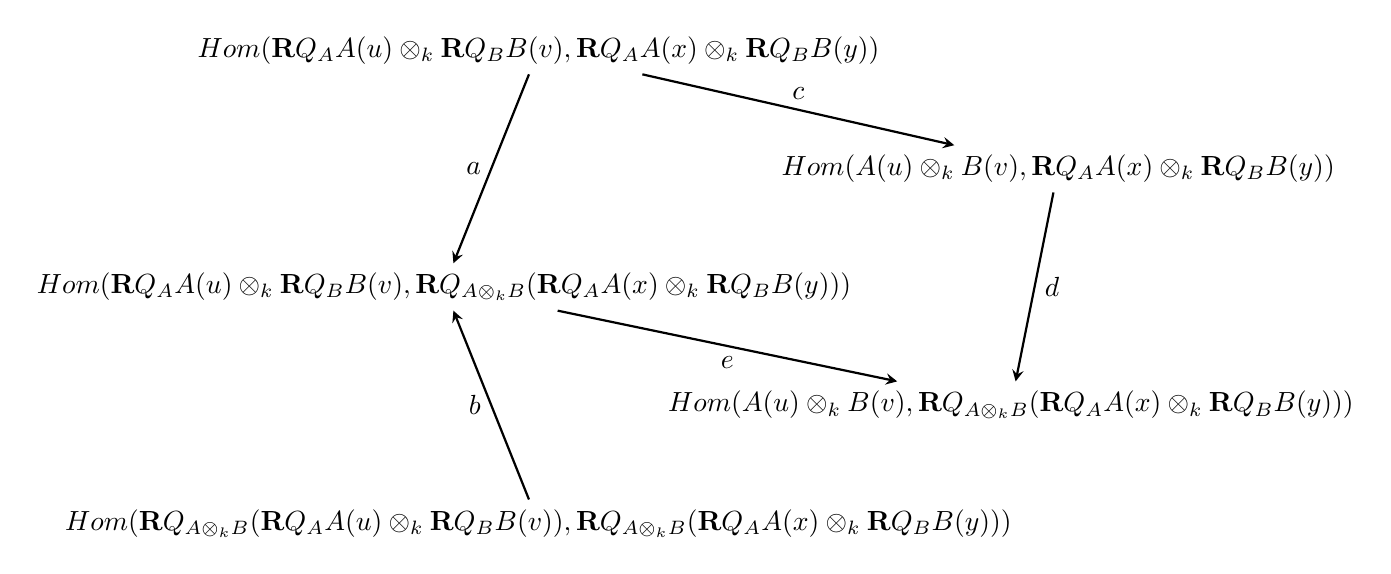
\begin{tikzpicture}[scale=.6,level/.style={->,>=stealth,thick}]
	\node (a) at (-5,5) {\(\op{Hom}(\mathbf{R} Q_A A(u) \otimes_k \mathbf{R} Q_B B(v),\mathbf{R} Q_A A(x) \otimes_k \mathbf{R} Q_B B(y))\)};
	\node (b) at (6,2.5) {\(\op{Hom}(A(u) \otimes_k B(v),\mathbf{R} Q_A A(x) \otimes_k \mathbf{R} Q_B B(y))\)};
	\node (c) at (-7,0) {\(\op{Hom}(\mathbf{R} Q_A A(u) \otimes_k \mathbf{R} Q_B B(v),\mathbf{R}Q_{A \otimes_k B} (\mathbf{R} Q_A A(x) \otimes_k \mathbf{R} Q_B B(y)))\)};
	\node (d) at (5,-2.5) {\(\op{Hom}(A(u) \otimes_k B(v),\mathbf{R}Q_{A \otimes_k B} (\mathbf{R} Q_A A(x) \otimes_k \mathbf{R} Q_B B(y)))\)};
	\node (e) at (-5,-5) {\(\op{Hom}(\mathbf{R}Q_{A \otimes_k B} (\mathbf{R} Q_A A(u) \otimes_k \mathbf{R} Q_B B(v)),\mathbf{R}Q_{A \otimes_k B} (\mathbf{R} Q_A A(x) \otimes_k \mathbf{R} Q_B B(y)))\)};
	\draw[level] (a) -- node[left] {\(a\)} (c) ;
	\draw[level] (e) -- node[left] {\(b\)} (c) ;
	\draw[level] (a) -- node[above] {\(c\)} (b) ;
	\draw[level] (b) -- node[right] {\(d\)} (d) ;
	\draw[level] (c) -- node[below] {\(e\)} (d) ;
    \end{tikzpicture} }
  \end{center}
  and we want to know first that \(a\) and \(b\) are quasi-isomorphisms. We know that \(b\) is a quasi-isomorphism since \(\mathbf{R}\tau_{A \otimes_k B}\) is left orthogonal to \(\mathbf{R}Q_{A \otimes_k B}\) so we only need to check \(a\). Since \(A(u) \otimes_k B(v)\) is free and 
  \begin{displaymath}
    \mathbf{R} Q_A A(u) \otimes_k \mathbf{R} Q_B B(v) \to \mathbf{R}Q_{A \otimes B} (\mathbf{R} Q_A A(u) \otimes_k \mathbf{R} Q_B B(v) )
  \end{displaymath}
  is a quasi-isomorphism, \(d\) is a quasi-isomorphism. Since \(\mathbf{R}Q_A\) and \(\mathbf{R}Q_B\) commute with coproducts, using tensor-Hom adjunction shows that \(c\) is a quasi-isomorphism. Finally, since the cone over the map
  \begin{displaymath}
    A(u) \otimes_k A(v) \to \mathbf{R} Q_A A(u) \otimes_k \mathbf{R} Q_B B(v)
  \end{displaymath}
  is annihilated by \(\tau_{A \otimes_k B}\), we see that \(e\) is also a quasi-isomorphism. This implies that \(a\) is a quasi-isomorphism.
  By an analogous argument, the endomorphisms of \(\mathbf{R}Q_{A \otimes B} (A(u) \otimes_k B(v))\) and \(\mathbf{R}Q_{A \otimes B} (\mathbf{R} Q_A A(u) \otimes_k \mathbf{R} Q_B B(v) )\) are quasi-isomorphic.
\end{proof}


\section{The quasi-equivalence}

Now we turn to the main result. 

\begin{theorem} \label{theorem: derived morita for NCP}
  Let \(k\) be a field. Let \(A\) and \(B\) be connected graded \(k\)-algebras. If \(A\) and \(B\) form a tasty pair, then there is a natural quasi-equivalence 
  \begin{displaymath}
    F : \hinj{\QGr{A^\opp \otimes_k B}} \to \RHomc{ \hinj{\QGr{A}}, \hinj{\QGr{B}} }
  \end{displaymath}
  such that for an object \(P\) of \(\mathrm{D}(\QGr{A^\opp \otimes_k B})\), the exact functor \(H^0(F(P))\) is isomorphic to 
  \begin{displaymath}
    \Phi_P(M) :=  \pi_B \left( \mathbf{R}\omega_{A^\opp \otimes_k B} P \overset{\mathbf{L}}{\otimes}_{\mathcal A} \mathbf{R}\omega_A M \right).
  \end{displaymath}
\end{theorem}

\begin{proof}
  Applying Corollary~\ref{corollary: Toen}, it suffices to provide a quasi-equivalence
  \begin{displaymath}
    G : \hinj{\QGr{A^\opp \otimes_k B}} \to \hproj{ (Q \mathcal A)^\opp \otimes_k Q \mathcal B}
  \end{displaymath}
  Using Corollary~\ref{corollary: duality is a duality}, we have a quasi-equivalence
  \begin{displaymath}
    \hproj{ (Q \mathcal A)^\opp \otimes_k Q \mathcal B} \cong \hproj{ Q \mathcal A^\opp \otimes_k Q \mathcal B}. 
  \end{displaymath}
  From Lemma~\ref{lemma: another model for QA otimes QB} we have a quasi-fully faithful functor 
  \begin{displaymath}
    Q \mathcal A^\opp \otimes_k Q \mathcal B \to \hinj{\QGr{A^\opp \otimes_k B}}. 
  \end{displaymath}
  This gives a functor 
  \begin{displaymath}
    \hinj{\QGr{A^\opp \otimes_k B}} \to \hproj{Q \mathcal A^\opp \otimes_k Q \mathcal B}
  \end{displaymath}
  which is a quasi-equivalence by a standard argument, see e.g. \parencite[Theorem 5.1]{Dyckerhoff11}.
  
  Tracing out the quasi-equivalences, one just needs to manipulate 
  \begin{align*}
    \op{Hom} (\mathbf{R}Q_A A(x)^\vee \otimes_k \mathbf{R}Q_B B(y), P) & \cong \op{Hom} ( \mathbf{R}Q_B B(y) , \op{Hom}( \mathbf{R}Q_A A(x)^\vee, \mathbf{R}\omega_{A^\opp \otimes_k B} P)) \\
    & \cong \op{Hom} ( \mathbf{R}Q_B B(y) , \mathbf{R}\omega_{A^\opp \otimes_k B} P \overset{\mathbf{L}}{\otimes}_{\mathcal A} \mathbf{R}Q_A A(x) ) 
  \end{align*}
  using Propostion~\ref{proposition: vanishing of tensor} and Lemma~\ref{lemma: trace map}. This says that the induced continuous functor is
  \begin{displaymath}
    M \mapsto \pi_B \left( \mathbf{R}\omega_{A^\opp \otimes_k B} P \overset{\mathbf{L}}{\otimes}_{\mathcal A} \mathbf{R}\omega_A M \right). 
  \end{displaymath}
\end{proof}

The following statement is now a simple application of Theorem~\ref{theorem: derived morita for NCP} and results of \parencite{Lunts-Orlov}. 

\begin{corollary} \label{corollary: NCP morita}
  Let \(A\) and \(B\) be a tasty pair of connected graded \(k\)-algebras with \(k\) a field. Assume that there exists an equivalence
  \begin{displaymath}
    f : \mathrm{D} (\QGr{A}) \to \mathrm{D} (\QGr{B}).
  \end{displaymath}
  Then there exists an object \(P \in D ( \QGr{A^\opp \otimes_k B} )\) such that 
  \begin{displaymath}
    \Phi_P : \mathrm{D} ( \QGr{A}) \to \mathrm{D} (\QGr{B} )
  \end{displaymath}
  is an equivalence.
\end{corollary}

\begin{proof}
  Applying \parencite[Theorem 1]{Lunts-Orlov} we know there is a quasi-equivalence between the unique enhancements, i.e. there is an \( F \in [ \hinj{ \QGr{A}}, \hinj{ \QGr{B}} ]\) giving an equivalence
  \begin{displaymath}
    H^0(F) : H^0(\hinj{ \QGr{A} }) = \mathrm{D}(\QGr{A}) \to H^0(\hinj{ \QGr{B} }) = \mathrm{D}(\QGr{B}).
  \end{displaymath}
  Then, by Theorem~\ref{theorem: derived morita for NCP}, there exists a \(P \in \mathrm{D}(\QGr{A^\opp \otimes_k B})\) such that \(\Phi_P = H^0(F)\). 
\end{proof}

We wish to identify the kernels as objects of the derived category of an honest noncommutative projective scheme.  Towards this end, we define a graded ring associated to a pair of graded \(k\)-algebras.
\begin{definition}\label{def: segre product}
  Let \(A\) and \(B\) be connected graded \(k\)-algebras.
  The \textbf{Segre product} of \(A\) and \(B\) is the graded \(k\)-algebra
  \[ A \times_k B = \bigoplus_{0 \leq i} A_i \otimes_k B_i.\]
\end{definition}

In general, one can only hope that kernels obtained as above are objects of the derived category of a noncommutative (bi)projective scheme.
However, we have the following special case in which we can collapse the \(\Z^2\)-grading to a \(\Z\)-grading.
Denote by \(\A \times \B\) the dg-category with objects \(\Z\) and morphisms \(\A \times \B(i,j)\) the chain complex with \(A_i \otimes_k B_i\) in degree zero.

\begin{lemma}\label{lemma: Q(AxB) is Q(A tensor B)}
  Assume \(A\) and \(B\) satisfy (insert hypotheses here).
  Then there is a quasi-equivalence
  \[Q(\A \times \B) \to Q(\A \otimes \B)\]
\end{lemma}

\begin{proof}
  We have an obvious functor \(\Delta \colon \A \times \B \to \A \otimes \B\) defined by \(\Delta(i) = (i,i)\) on objects with structure morphism the identity.
  %\[ \A \times \B(i,j) = A_{j-i} \otimes_k B_{j-i} \to A_{j-i} \otimes_k B_{j-i}= \A \otimes \B((i,i), (j,j)).\]
  This yields an adjoint pair of dg-functors \(\Ind{\Delta} \colon \dgMod{\A \times \B} \to \dgMod{\A \otimes \B}\) and \(\Res{\Delta} \colon \dgMod{\A \otimes \B} \to \dgMod{\A \times \B}\).
  Moreover, it is easy to check that \(\Ind{\Delta}\) is induced by the object \(P\) of \(\dgMod{\left(\A \times \B\right)^\opp \otimes \left(\A \otimes \B \right)}\) defined by
  \[P(i,(m,n)) = \left(\A \otimes \B\right)^\opp\left((i,i),(m,n)\right) = A_{i- m} \otimes_k B_{i - n}\]
  in the sense that \(\Ind{\Delta} \cong \widehat{\Phi_P} = - \otimes_{\A \times \B} P\).
\end{proof}
\begin{corollary} \label{corollary: NCP morita degree 1}
  Let \(A\) and \(B\) be a tasty pair of connected graded \(k\)-algebras with \(k\) a field that are both generated in degree one.
  Assume that there exists an equivalence
  \begin{displaymath}
    f : \mathrm{D} (\QGr{A}) \to \mathrm{D} (\QGr{B}).
  \end{displaymath}
  Then there exists an object \(P \in D ( \QGr{A^\opp \times_k B} )\) such that 
  \begin{displaymath}
    \Phi_P : \mathrm{D} ( \QGr{A}) \to \mathrm{D} (\QGr{B} )
  \end{displaymath}
  is an equivalence.
\end{corollary}

\begin{proof}
\end{proof}
